\documentclass{report}
\usepackage[a4paper, total={7.5in, 10in}]{geometry}
\usepackage[fleqn]{amsmath}
\usepackage{amssymb}
\usepackage{amsthm}
\usepackage{enumitem}
\usepackage[]{mdframed}
\usepackage{multicol}
\usepackage{thmtools}
\usepackage{graphicx}
\usepackage{tikz}
\usepackage{tipa}
\usepackage{array, makecell, cellspace}
\usepackage{bigints}
\usepackage[export]{adjustbox}
\setlength{\cellspacetoplimit}{13.2ex}
\setlength{\cellspacebottomlimit}{13.2ex}

\usepackage{ifxetex}

\ifxetex
      \usepackage{substitutefont}
      \substitutefont{T3}{\rmdefault}{cmr}
\fi

\usepackage{fontspec}
\setmainfont[Mapping=tex-text]{Georgia}

\title{Praktis 3\\Integration}
\author{Melvin Chia}

\newcommand{\sol}[1]{

      \noindent \textbf{Sol.}
}
\newcommand{\prooff}[1]{

      \noindent \textbf{Proof.}
}

\newcommand{\arc}[1]{{%
                  \setbox9=\hbox{#1}%
                  \ooalign{\resizebox{\wd9}{\height}{\texttoptiebar{\phantom{A}}}\cr#1}}}

\def\eos{\quad\hbox{\rlap{\hbox{\vrule depth 1.5pt height 2.6mm width 0.2mm \hskip 1mm \vrule height 2.6mm width 0.2mm}}{\vbox{\hrule height 0.2mm width 1.4mm \vskip 2.8mm \hrule depth 1.5pt height -0.35mm width 1.2mm}}}}

\counterwithout{equation}{chapter}
\setlength{\columnseprule}{1pt}
\setlength{\columnsep}{24pt}
\hfuzz=100pt
\setcounter{chapter}{3}

\begin{document}
\maketitle

\begin{multicols*}{2}
      \noindent\Large{\underline{\textbf{Praktis Formatif}}}
      \normalsize
      \section{Integration as the Inverse of Differentiation}
      \begin{enumerate}
            \item \begin{enumerate}
                        \item Given ${\dfrac{d}{d x}}(2x^{3}+5x^{2}-7x)=6x^{2}+ 10x - 7$, find $\displaystyle
                                    \int6x^{2}+10x-7\ d x$. \sol{}
                              \begin{flalign*}
                                    \int6x^{2}+10x-7\ dx & = 2x^{3}+5x^{2}-7x \eos
                              \end{flalign*}

                        \item Given ${\dfrac{d}{d x}}(5x^{4}+3x^{2}+x)=20x^{3}+6x+1$, find $\displaystyle
                                    \int20x^{3}+6x+1\ dx$. \sol{}
                              \begin{flalign*}
                                    \int20x^{3}+6x+1\ dx & = 5x^{4}+3x^{2}+x \eos
                              \end{flalign*}
                  \end{enumerate}

            \item \begin{enumerate}
                        \item Given ${\dfrac{d}{d x}}(4x-5x^{2}+2x^{3})=4-10x+6x^{2}$, find $\displaystyle
                                    \int2-5x+3x^{2}\ dx$. \sol{}
                              \begin{flalign*}
                                    \int2-5x+3x^{2}\ dx & = \frac{2}{2}\int2-5x+3x^{2}\ dx    \\
                                                        & = \frac{1}{2} \int 4-10x+6x^{2}\ dx \\
                                                        & = \frac{1}{2}(4x-5x^{2}+2x^{3})     \\
                                                        & = 2x-\frac{5}{2}x^{2}+x^{3} \eos
                              \end{flalign*}

                        \item Given $\dfrac{d}{d x}\Big(2x-{\dfrac{3}{x^{4}}}\Big)=2+{\dfrac{12}{x^{5}}}$,
                              find $\displaystyle \int 6+{\dfrac{36}{x^{5}}}\ dx$ \sol{}
                              \begin{flalign*}
                                    \int 6+{\dfrac{36}{x^{5}}}\ dx & = 6\int 1+{\dfrac{6}{x^{5}}}\ dx       \\
                                                                   & = 3\int 2+{\dfrac{12}{x^{5}}}\ dx      \\
                                                                   & 3\left(2x-{\dfrac{3}{x^{4}}}   \right) \\
                                                                   & = 6x-{\dfrac{9}{x^{4}}} \eos
                              \end{flalign*}

                        \item Given $f(x)={\dfrac{d}{d x}}[g(x)]$, find $\displaystyle \int 2f(x)\,d x$.
                              \sol{}
                              \begin{flalign*}
                                    \int 2f(x)\,dx & = 2\int f(x)\,dx \\
                                                   & = 2g(x) \eos
                              \end{flalign*}

                        \item Differentiate $\dfrac{2x^{2}}{3x-1}$ with respect to $x$ and hence, find
                              $\displaystyle \int{\dfrac{6x(3x-2)}{{(3x-1)}^{2}}}\,d x$. \sol{}
                              \begin{flalign*}
                                    \frac{d}{dx}\left(\dfrac{2x^{2}}{3x-1}\right) & = \frac{4x(3x-1) - 3(2x^2)}{{(3x-1)}^2}  \\
                                                                                  & = \frac{12x^2 - 4x - 6x^2}{{(3x-1)}^2}   \\
                                                                                  & = \frac{6x^2 - 4x}{{(3x-1)}^2}           \\
                                                                                  & = \frac{2x(3x-2)}{{(3x-1)}^2}            \\
                                    \int{\dfrac{6x(3x-2)}{{(3x-1)}^{2}}}\,d x     & = 3\int \frac{2x(3x-2)}{{(3x-1)}^2}\,d x \\
                                                                                  & = 3\left(\dfrac{2x^2}{3x-1}\right)       \\
                                                                                  & = \dfrac{6x^2}{3x-1} \eos
                              \end{flalign*}
                  \end{enumerate}

            \item The daily production of bread of a bakery shop is given b y the function $R(x)
                        = -50(x^2 - 12x)$, where $x$ represents the number of bakers who work in the
                  shop with condition $x$ is not more than 6.
                  \begin{enumerate}
                        \item Find the rate of daily production of bread in terms of $x$. \sol{}
                              \begin{flalign*}
                                    R'(x) & = -100x + 600 \eos
                              \end{flalign*}

                        \item If the rate of daily production of bread becomes $300 - 50x$ on a particular
                              day, calculate the revenue of the bakery shop if all the loaves of bread baked
                              by three bakers on that day are sold out at a price of RM$5.50$ for each loaf.
                              \sol{}
                              \begin{flalign*}
                                    \int 300 - 50x\ dx & = \frac{1}{2}\int (600 - 100x)\ dx \\
                                                       & = \frac{1}{2}(-50x^2 + 600x)       \\
                                                       & = -25x^2 + 300x                    \\
                                    R(3)               & = -25{(3)}^2 + 300(3)              \\
                                                       & = -225 + 900                       \\
                                                       & = 675
                              \end{flalign*}
                              \begin{flalign*}
                                    \text{Revenue} & = 675 \times 5.50       \\
                                                   & = \text{RM}3712.50 \eos
                              \end{flalign*}
                  \end{enumerate}

            \item Given $f(x) = x^4 - 2x^3$ and $f'(x) = 4x^3 - 6x^2$. Express
                  $f'(x)\displaystyle \int f'(x)\,dx$ in factored form. \sol{}
                  \begin{flalign*}
                        f'(x)\displaystyle \int f'(x)\,dx & = (4x^3 - 6x^2)(x^4 - 2x^3) \\
                                                          & = 2x^5(2x - 3)(x - 2) \eos
                  \end{flalign*}

            \item Given $y=\dfrac{2x-6}{x}$.
                  \begin{enumerate}
                        \item Find $\dfrac{dy}{dx}$. \sol{}
                              \begin{flalign*}
                                    \frac{dy}{dx} & = \frac{2x - 2x-6}{x^2} \\
                                                  & = -\frac{6}{x^2} \eos
                              \end{flalign*}

                        \item Solve $4+\displaystyle \int\left(\dfrac{dy}{dx}\right)\,dx=0$. \sol{}
                              \begin{flalign*}
                                    4+\displaystyle \int\left(\dfrac{dy}{dx}\right)\,dx=0 \\
                                    4+\displaystyle \int\left(-\frac{6}{x^2}\right)\,dx=0 \\
                                    4 + \frac{2x-6}{x} & = 0                              \\
                                    4x + 2x - 6        & = 0                              \\
                                    6x                 & = 6                              \\
                                    x                  & = 1 \eos
                              \end{flalign*}
                  \end{enumerate}

            \item Given $f'(x) = g(x)$. Find ${\dfrac{3f(x)}{\displaystyle \int g(x)dx}}$. \sol{}
                  \begin{flalign*}
                        f'(x)                                      & = g(x)                      \\
                        f(x)                                       & = \displaystyle \int g(x)dx \\
                        {\dfrac{3f(x)}{\displaystyle \int g(x)dx}} & = \frac{3f(x)}{f(x)}        \\
                                                                   & = 3 \eos
                  \end{flalign*}

            \item The population of town $A$ is given by a function $P(t) =
                        \dfrac{5}{6}(2.72^{1.2t}) - t^2 + 1495$ and the population continues to
                  increase at the rate of $2.72^{1.2t} - 2t$ people per year where $t$ is the
                  number of years. Given that the population of town $b$ increases at twice the
                  rate of the population of town $A$ based on the same model, find, to the
                  nearest integer,
                  \begin{enumerate}
                        \item the rate of increase of the population of town $B$ at $t=5$ years. \sol{}
                              \begin{flalign*}
                                    P_B'(5) & = 2[2.72^{1.2(5)} - 2(5)]          \\
                                            & = 2[404.96 - 10]                   \\
                                            & = 2(394.96)                        \\
                                            & = 789.92                           \\
                                            & = 790 \text{ people per year} \eos
                              \end{flalign*}

                        \item the population of town $B$ after 5 years. \sol{}
                              \begin{flalign*}
                                    P_B(5) & = 2\left[\dfrac{5}{6}(2.72^{1.2\cdot 5}) - {(5)}^2 + 1495\right] \\
                                           & = \frac{5}{3}(2.72^{6}) - 50 + 2990                              \\
                                           & = 3614.93                                                        \\
                                           & = 3615 \text{ people} \eos
                              \end{flalign*}
                  \end{enumerate}
      \end{enumerate}

      \section{Indefinite Integral}
      \begin{enumerate}
            \setcounter{enumi}{7}

            \item By using the indefinite integral formula, find the integral of each of the
                  following constants or algebraic functions.
                  \begin{enumerate}
                        \item $\displaystyle \int 3\,dx$
                              \sol{}
                              \begin{flalign*}
                                    \int 3\,dx & = 3x + C \eos
                              \end{flalign*}

                        \item $\displaystyle \int 24x\,dx$
                              \sol{}
                              \begin{flalign*}
                                    \int 24x\,dx & = 12x^2 + C \eos
                              \end{flalign*}

                        \item $\displaystyle \int 6x^{2}\,dx$
                              \sol{}
                              \begin{flalign*}
                                    \int 6x^{2}\,dx & = 2x^3 + C \eos
                              \end{flalign*}

                        \item $\displaystyle \int 3x^2 + 4x\,dx$
                              \sol{}
                              \begin{flalign*}
                                    \int 3x^2 + 4x\,dx & = x^3 + 2x^2 + C \eos
                              \end{flalign*}

                        \item $\displaystyle \int \dfrac{2}{x^4}\,dx$
                              \sol{}
                              \begin{flalign*}
                                    \int \dfrac{2}{x^4}\,dx & = -\dfrac{2}{x^3} + C \eos
                              \end{flalign*}

                        \item $\displaystyle \int x^2(x-3)\,dx$
                              \sol{}
                              \begin{flalign*}
                                    \int x^2(x-3)\,dx & = \int x^3-3x^2\,dx             \\
                                                      & = \frac{1}{4}x^4 - x^3 + C \eos
                              \end{flalign*}

                        \item $\displaystyle \int (x+2)(2x^4 - 1)\,dx$
                              \sol{}
                              \begin{flalign*}
                                     & \int (x+2)(2x^4 - 1)\,dx                                           \\
                                     & = \int 2x^5 - x + 4x^4 - 2                                       & \\
                                     & = \frac{1}{3}x^6 + \frac{4}{5}x^5 - \frac{1}{2}x^2 - 2x + C \eos
                              \end{flalign*}

                        \item $\displaystyle \int \dfrac{x^2 + 3x + 2}{x+2}\,dx$
                              \sol{}
                              \begin{flalign*}
                                    \displaystyle \int \dfrac{x^2 + 3x + 2}{x+2}\,dx & = \displaystyle \int \dfrac{(x+2)(x+1)}{x+2}\,dx \\
                                                                                     & = \displaystyle \int x+1\,dx                     \\
                                                                                     & = \frac{1}{2}x^2 + x + C \eos
                              \end{flalign*}
                  \end{enumerate}

            \item Find the indefinite integral for each of the following by using
                  \begin{enumerate}
                        \item the substitution method.
                        \item the indefinite integral formula.
                  \end{enumerate}
                  \begin{enumerate}[label=\roman*.]
                        \item $\displaystyle \int{\dfrac{2}{{(x+2)}^{5}}}\,d x$
                              \sol{}
                              \begin{enumerate}[label=(\alph*)]
                                    \item Let $v = {(x+2)}$.
                                          \begin{flalign*}
                                                \int{\dfrac{2}{{(x+2)}^{5}}}\,d x & = \int{\dfrac{2}{v^5}}\,dv       \\
                                                                                  & = \int 2v^{-5}\,dv               \\
                                                                                  & = -\frac{1}{2}v^{-4} + C         \\
                                                                                  & = -\frac{1}{2v^4} + C            \\
                                                                                  & = -\frac{1}{2{(x+2)}^4} + C \eos
                                          \end{flalign*}

                                    \item \begin{flalign*}
                                                \int{\dfrac{2}{{(x+2)}^{5}}}\,d x & = \int2{(x+2)}^{-5}\,dx                     \\
                                                                                  & = 2\int{(x+2)}^{-5}\,dx                     \\
                                                                                  & = 2\left[\frac{{(x+2)}^{-4}}{-4}\right] + C \\
                                                                                  & = -\frac{1}{2{(x+2)}^4} + C \eos
                                          \end{flalign*}
                              \end{enumerate}

                        \item $\displaystyle \int{\dfrac{3}{5}{(3x+2)}^8}\,d x$
                              \sol{}
                              \begin{enumerate}[label=(\alph*)]
                                    \item Let $v = 3x+2$, $\dfrac{dv}{dx} = 3$.
                                          \begin{flalign*}
                                                \int{\dfrac{3}{5}{(3x+2)}^8}\,d x & = \int{\dfrac{3}{5}v^8}\,dv         \\
                                                                                  & = \int{\dfrac{3}{5}v^8}\frac{dv}{3} \\
                                                                                  & = \int{\dfrac{1}{5}v^8}\,dv         \\
                                                                                  & = \dfrac{1}{45}v^9 + C              \\
                                                                                  & = \dfrac{(3x+2)^9}{45} + C \eos
                                          \end{flalign*}

                                    \item \begin{flalign*}
                                                \int{\dfrac{3}{5}{(3x+2)}^8}\,d x & = \dfrac{3}{5}\int{(3x+2)^8}\,dx                     \\
                                                                                  & = \dfrac{3}{5}\left[\frac{{(3x+2)}^9}{27}\right] + C \\
                                                                                  & = \dfrac{{(3x+2)}^9}{45} + C \eos
                                          \end{flalign*}
                              \end{enumerate}
                  \end{enumerate}

            \item Determine the equation of a curve based on the following information.
                  \begin{enumerate}
                        \item The gradient function of the curve is $\dfrac{dy}{dx} = 3x^2 + x - 2$ and it
                              passes through the point $p(2, 15)$. \sol{}
                              \begin{flalign*}
                                    \dfrac{dy}{dx} & = 3x^2 + x - 2                 \\
                                    y              & = \int 3x^2 + x - 2\,dx        \\
                                                   & = x^3 + \frac{x^2}{2} - 2x + C \\
                              \end{flalign*}
                              When $x = 2$, $y = 15$,
                              \begin{flalign*}
                                    15 & = 2^3 + \frac{2^2}{2} - 2(2) + C \\
                                    15 & = 8 + 2 - 4 + C                  \\
                                    15 & = 6 + C                          \\
                                    C  & = 9
                              \end{flalign*}
                              Hence, the equation of the curve is $y = x^3 + \dfrac{x^2}{2} - 2x + 9$. $\eos$

                        \item The gradient function of the curve is $f'(x) = 2x+9$ and $f(3) = 21$. \sol{}
                              \begin{flalign*}
                                    f'(x) & = 2x+9           \\
                                    f(x)  & = \int 2x+9\,dx  \\
                                          & = x^2 + 9x + C   \\
                                    f(3)  & = 3^2 + 9(3) + C \\
                                    21    & = 9 + 27 + C     \\
                                    C     & = -15
                              \end{flalign*}
                              Hence, the equation of the curve is $f(x) = x^2 + 9x - 15$. $\eos$

                        \item The gradient function of the curve is given by $g(t) = \dfrac{5t^2 - 6t +
                                          1}{t^3(t-1)}$ and it passes through the point $(1, 3)$. \sol{}
                              \begin{flalign*}
                                    g(t) & = \dfrac{5t^2 - 6t + 1}{t^3(t-1)}   \\
                                         & = \dfrac{(5t-1)(t-1)}{t^3(t-1)}     \\
                                         & = \dfrac{5t-1}{t^3}                 \\
                                         & = \dfrac{5}{t^2} - \dfrac{1}{t^3}   \\
                                         & = 5t^{-2} - t^{-3}                  \\
                                    f(t) & = \int 5t^{-2} - t^{-3}\,dt         \\
                                         & = -\frac{5}{t} + \frac{1}{2t^2} + C \\
                              \end{flalign*}
                              When $t = 1$, $f(1) = 3$,
                              \begin{flalign*}
                                    3 & = -5 + \frac{1}{2} + C \\
                                    3 & = -\frac{9}{2} + C     \\
                                    C & = \frac{15}{2}
                              \end{flalign*}
                              Hence, the equation of the curve is $f(t) = -\dfrac{5}{t} + \dfrac{1}{2t^2} + \dfrac{15}{2}$. $\eos$
                  \end{enumerate}

            \item Tommy moves in his roller skates at the rate of change in displacement,
                  $\dfrac{ds}{dt} = t^2 + 9$ metres per second, where $t$ is the time in seconds.
                  At $t = 3$ seconds, Tommy is 4 metres away from his starting place. Find the
                  displacement, $s$ metres, when $t = 10$ seconds. \sol{}
                  \begin{flalign*}
                        \frac{ds}{dt} & = t^2 + 9                \\
                        s             & = \int t^2 + 9\,dt       \\
                                      & = \frac{t^3}{3} + 9t + C
                  \end{flalign*}
                  When $t = 3$, $s = 4$,
                  \begin{flalign*}
                        4 & = \frac{3^3}{3} + 9(3) + C \\
                        4 & = 9 + 27 + C               \\
                        4 & = 54 + C                   \\
                        C & = -32                      \\
                        s & = \frac{t^3}{3} + 9t - 32
                  \end{flalign*}
                  When $t = 10$,
                  \begin{flalign*}
                        s & = \frac{10^3}{3} + 9(10) - 32   \\
                          & = 333 + 90 - 32                 \\
                          & = 391\frac{1}{3}\textit{m} \eos
                  \end{flalign*}

            \item Given the gradient function of a curve is $\dfrac{dy}{dx} = kx^2 + 2x$ where
                  $k$ is a constant. The curve passes through point $A(1, 6)$ and point $B(-2,
                        0)$. Determine the equation of the curve.
      \end{enumerate}

      \section{Definite Integral}
      \begin{enumerate}
            \setcounter{enumi}{12}
            \item Calculate each of the following.
                  \begin{enumerate}
                        \item $\displaystyle \int_{2}^{1}{\left(\sqrt{x} + \dfrac{1}{x}\right)}$
                        \item $\displaystyle \int_{0}^{3}\left(\dfrac{x^4 + 3x}{x}\right)\,dx$
                        \item $\displaystyle \int_{-2}^{-1}\left(\dfrac{(4-x)(3-x)}{x^5}\right)\,dx$
                  \end{enumerate}

            \item Given $\displaystyle \int_{a}^{b}f(x)\,dx = 5$, $\displaystyle
                        \int_{b}^{c}f(x)\,dx = 8$ and $\displaystyle \int_{b}^{a}g(x)\,dx = 2$. Find
                  each of the following.

                        [answer can be in terms of $a$ and/or $b$.]
                  \begin{enumerate}
                        \item $\displaystyle \int_{a}^{b}3f(x)\,dx$
                        \item $\displaystyle \int_{a}^{c}f(x)\,dx$
                        \item $\displaystyle \int_{a}^{b}[f(x) + g(x)]\,dx$
                        \item $\displaystyle \int_{c}^{a}f(x)\,dx$
                        \item $\displaystyle \int_{a}^{b}[g(x) + 3]\,dx$
                        \item $\displaystyle \int_{a}^{a}f(x)\,dx$
                        \item The value of $k$ such that $\displaystyle \int_{b}^{a}[f(x) + kx]\,dx = 25$ if
                              $a = 1$ and $b = 4$.
                  \end{enumerate}

            \item Find the area of the shaded region for each of the following diagrams.
                  \begin{enumerate}
                        \item 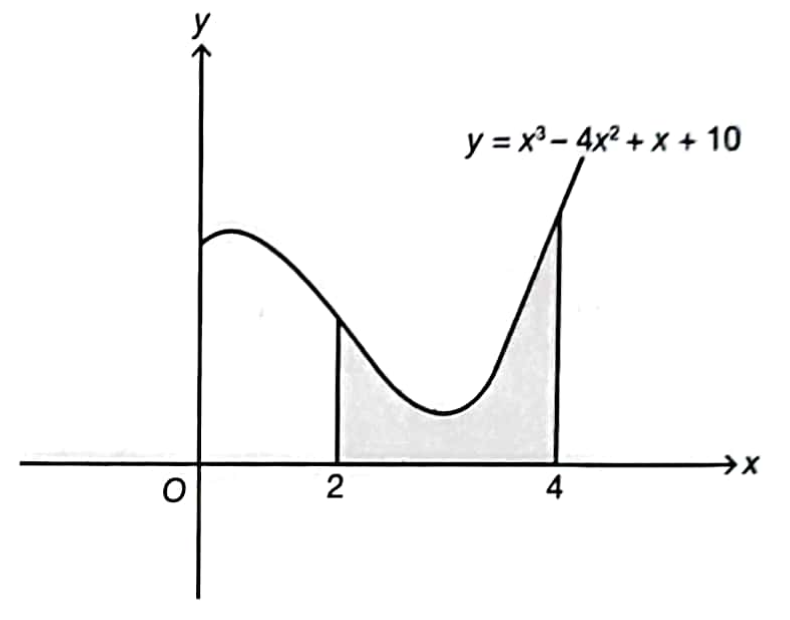
\includegraphics[width=0.3\textwidth,valign=t]{./images/1.png}
                        \item 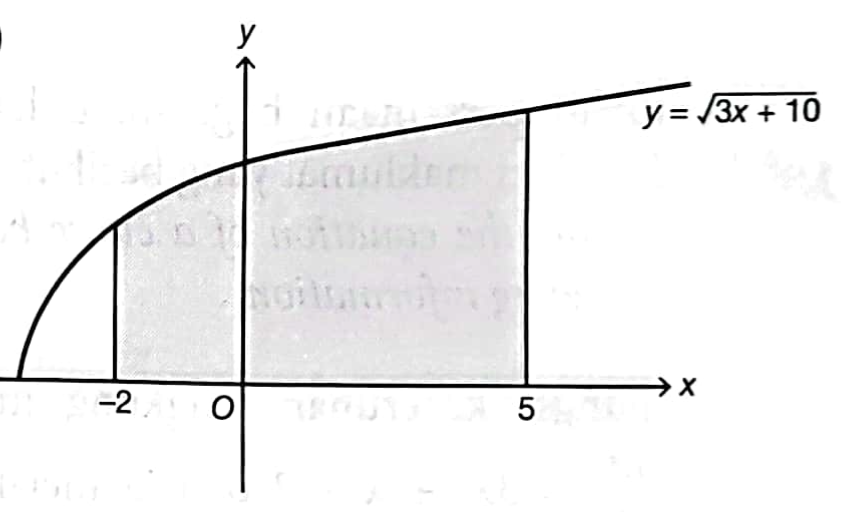
\includegraphics[width=0.3\textwidth,valign=t]{./images/2.png}
                        \item 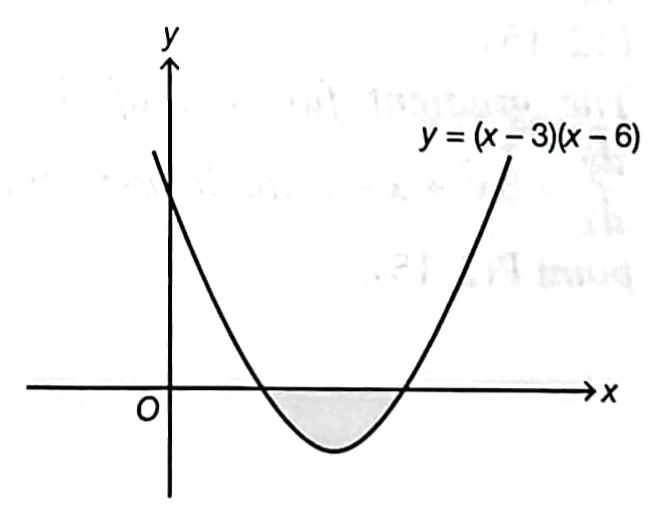
\includegraphics[width=0.3\textwidth,valign=t]{./images/3.png}
                        \item 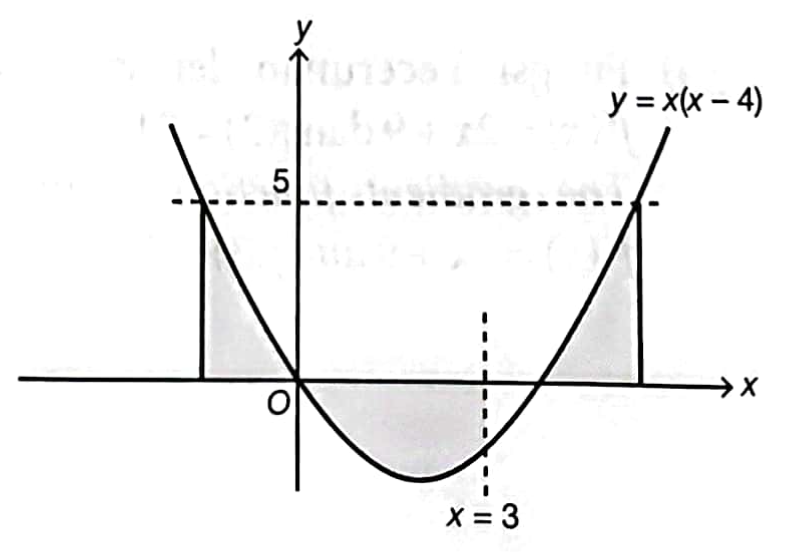
\includegraphics[width=0.3\textwidth,valign=t]{./images/4.png}
                  \end{enumerate}

            \item Determine the area bounded by the curve, the horizontal line(s) and the y-axis.
                  \begin{enumerate}
                        \item 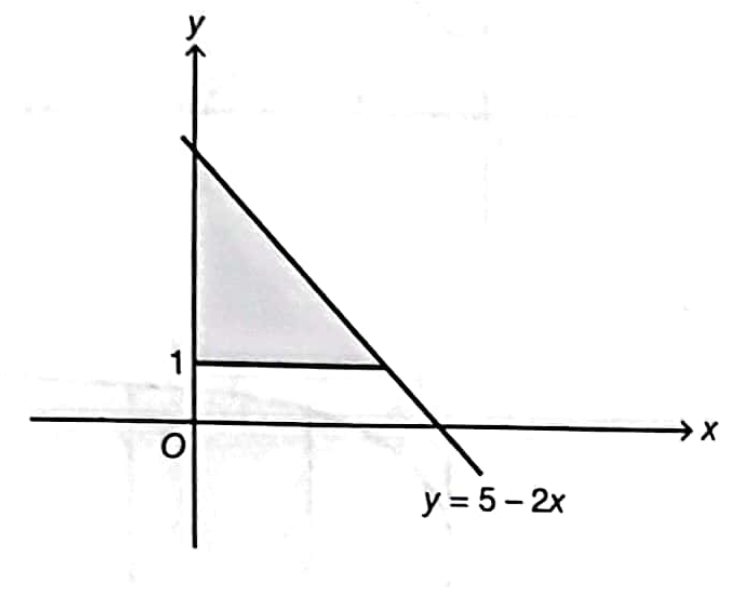
\includegraphics[width=0.3\textwidth,valign=t]{./images/5.png}
                        \item 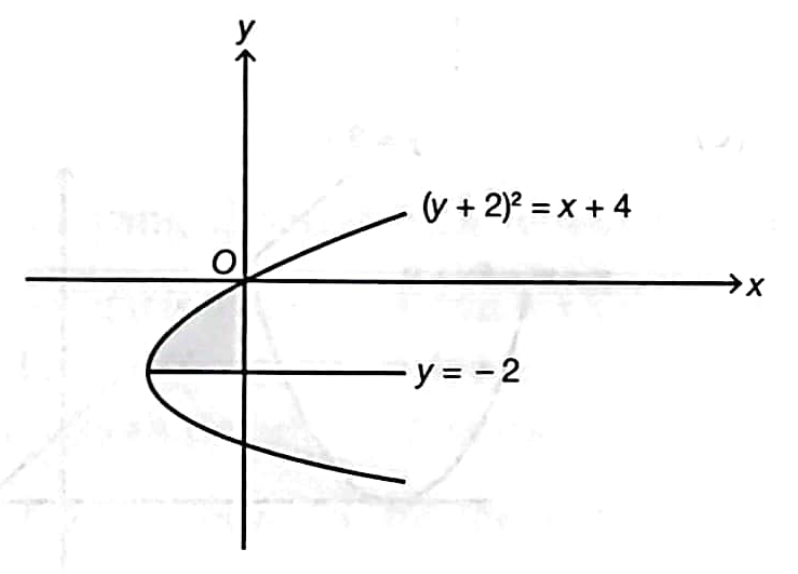
\includegraphics[width=0.3\textwidth,valign=t]{./images/6.png}
                        \item 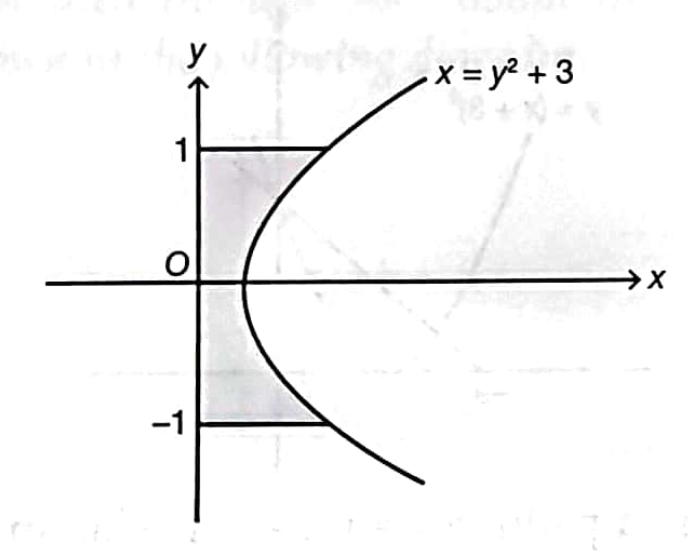
\includegraphics[width=0.3\textwidth,valign=t]{./images/7.png}
                        \item 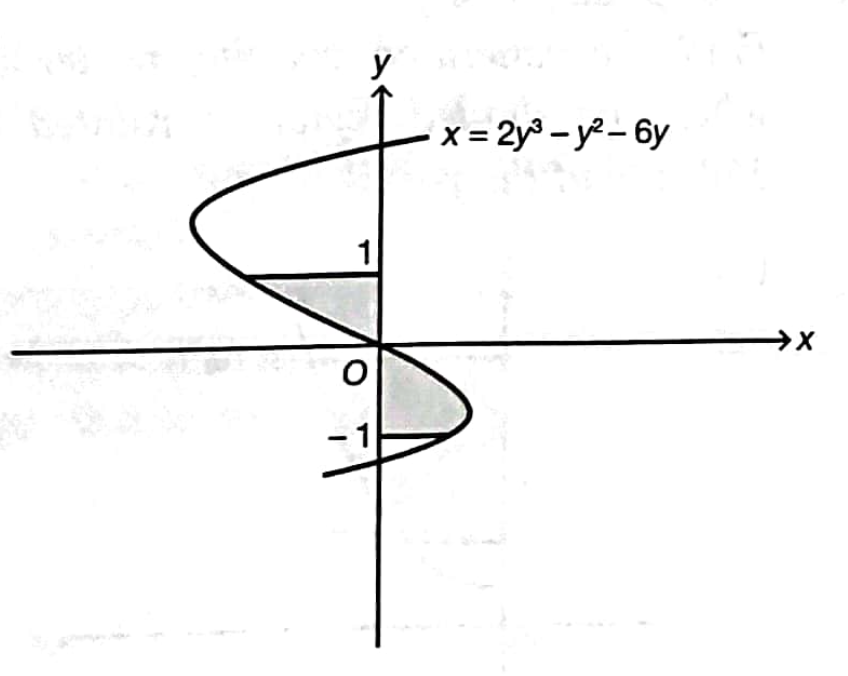
\includegraphics[width=0.3\textwidth,valign=t]{./images/8.png}
                  \end{enumerate}

            \item Find the area of the shaded region for each of the following.
                  \begin{enumerate}
                        \item 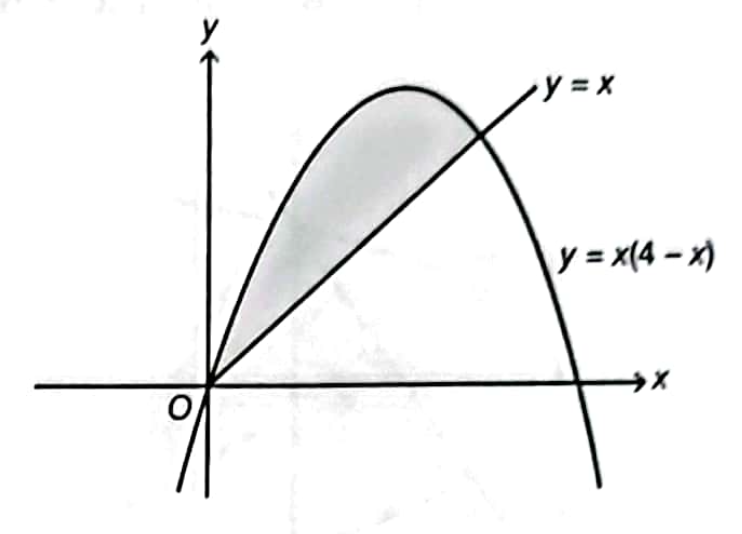
\includegraphics[width=0.3\textwidth,valign=t]{./images/9.png}
                        \item 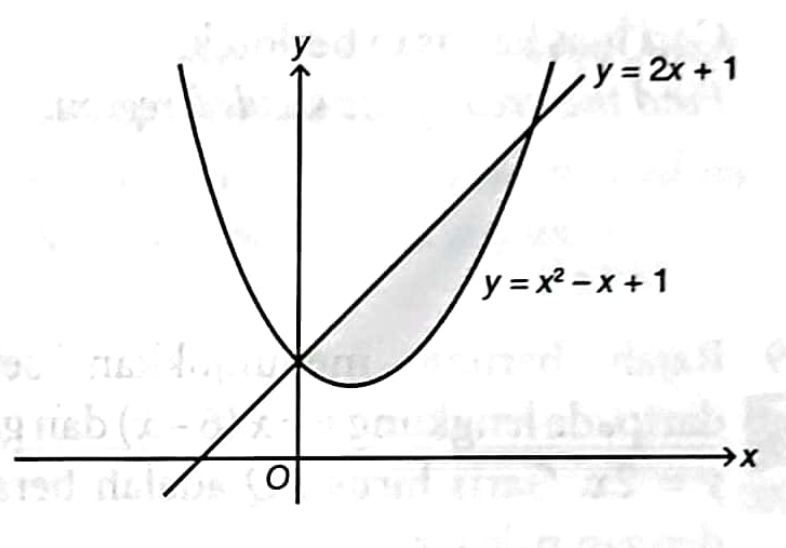
\includegraphics[width=0.3\textwidth,valign=t]{./images/10.png}
                        \item 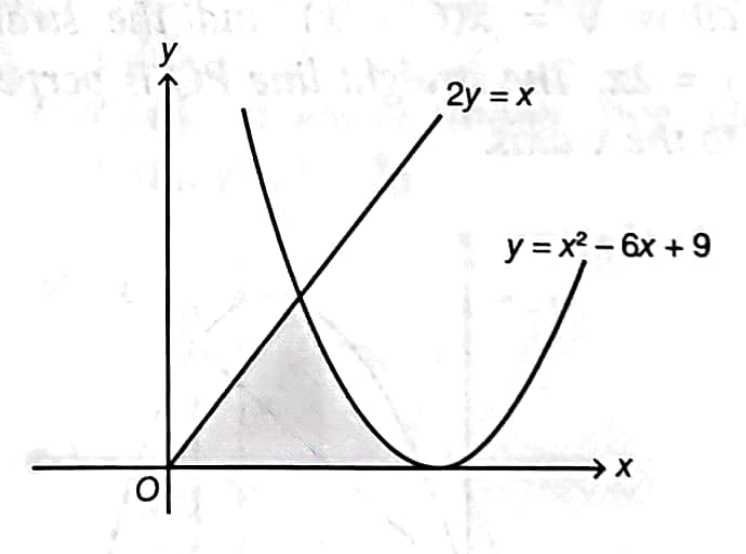
\includegraphics[width=0.3\textwidth,valign=t]{./images/11.png}
                        \item 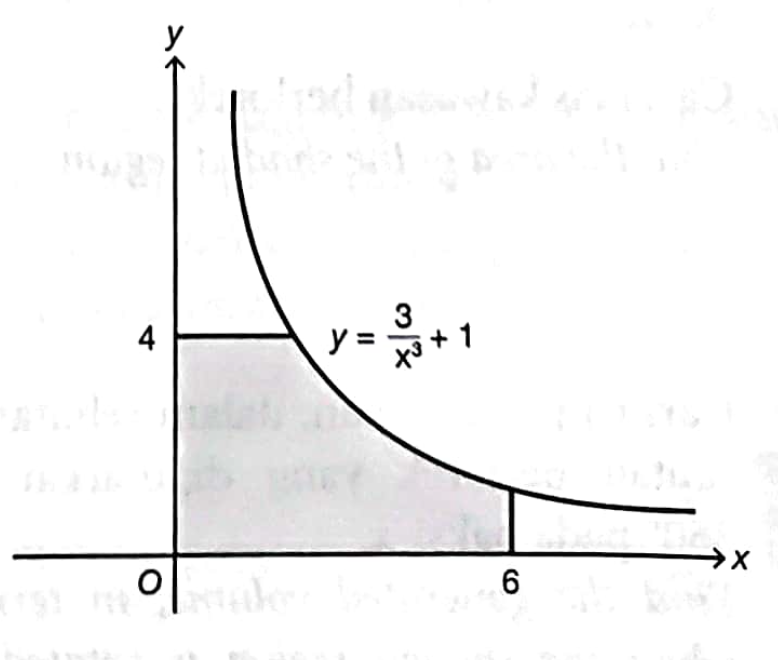
\includegraphics[width=0.3\textwidth,valign=t]{./images/12.png}
                  \end{enumerate}

            \item The following diagram shows a part of the curve $x = y(y-6)$ and the straight
                  line $y = x+6$.
                  \begin{center}
                        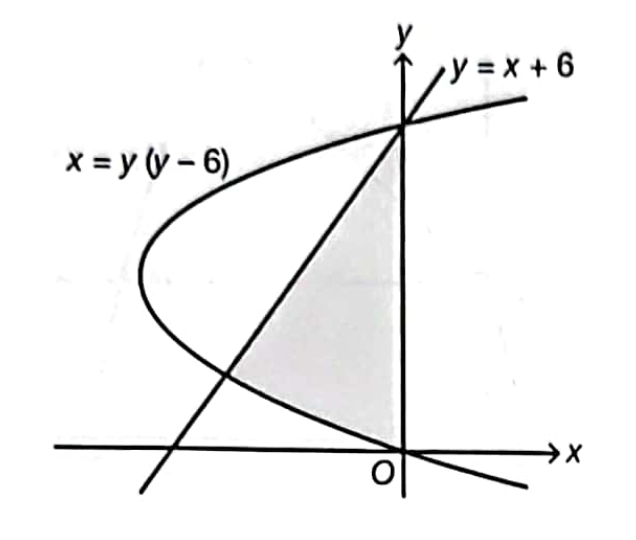
\includegraphics[width=0.3\textwidth,valign=t]{./images/13.png}
                  \end{center}
                  Find the area of the shaded region.

            \item The following diagram shows a part of the curve $y = x(6-x)$ and a straight
                  line $y = 2x$. The straight line $PQ$ is perpendicular to the x-axis.
                  \begin{center}
                        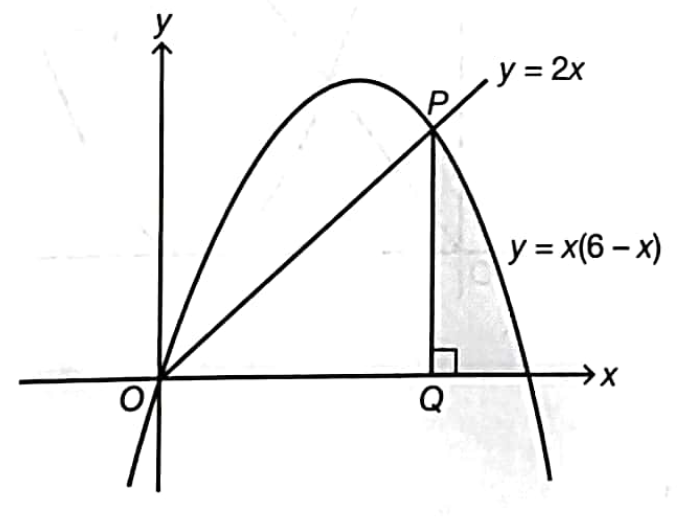
\includegraphics[width=0.3\textwidth,valign=t]{./images/14.png}
                  \end{center}
                  Find the area of the shaded region.

            \item Find the generated volume, in terms of $\pi$, when the shaded region is rotated
                  through $360^{\circ}$ about the $x$-axis.
                  \begin{enumerate}
                        \item 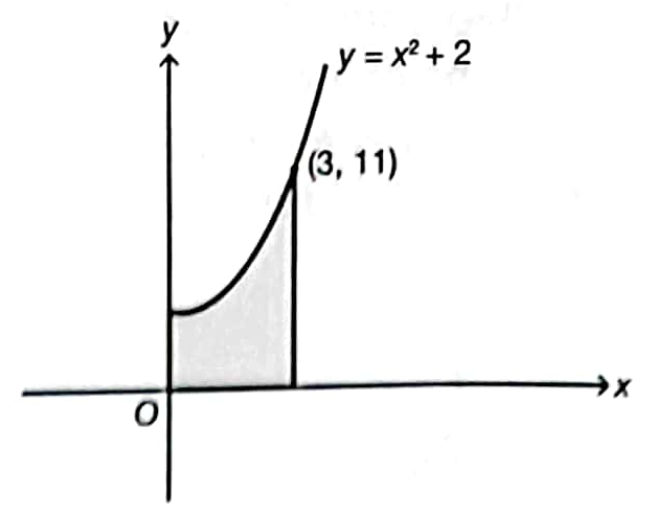
\includegraphics[width=0.3\textwidth,valign=t]{./images/15.png}
                        \item 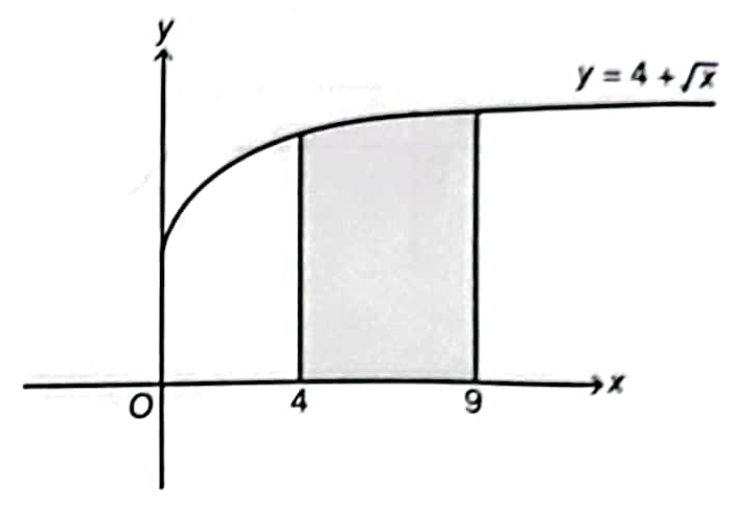
\includegraphics[width=0.3\textwidth,valign=t]{./images/16.png}
                        \item 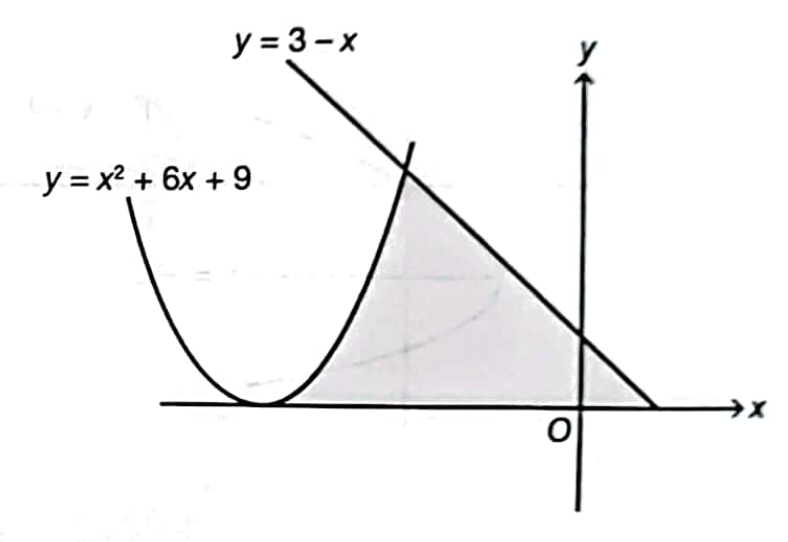
\includegraphics[width=0.3\textwidth,valign=t]{./images/17.png}
                        \item 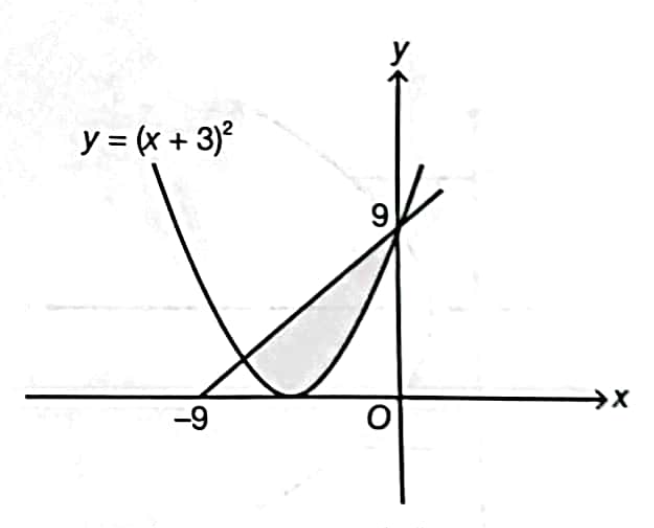
\includegraphics[width=0.3\textwidth,valign=t]{./images/18.png}
                  \end{enumerate}

            \item Find the generated volume, in terms of $\pi$, when the shaded region is rotated
                  through $360^\circ$ about the y-axis.
                  \begin{enumerate}
                        \item 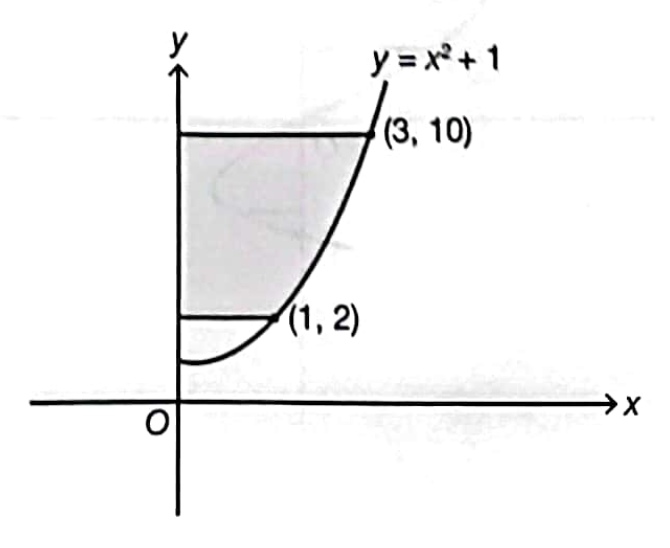
\includegraphics[width=0.3\textwidth,valign=t]{./images/19.png}
                        \item 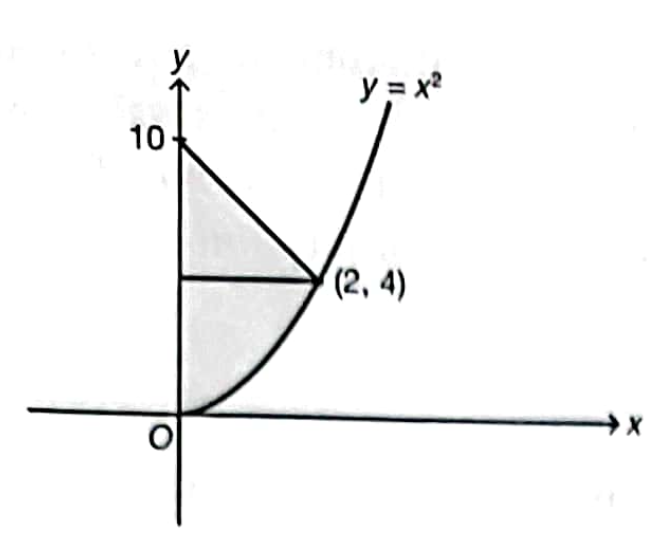
\includegraphics[width=0.3\textwidth,valign=t]{./images/20.png}
                        \item 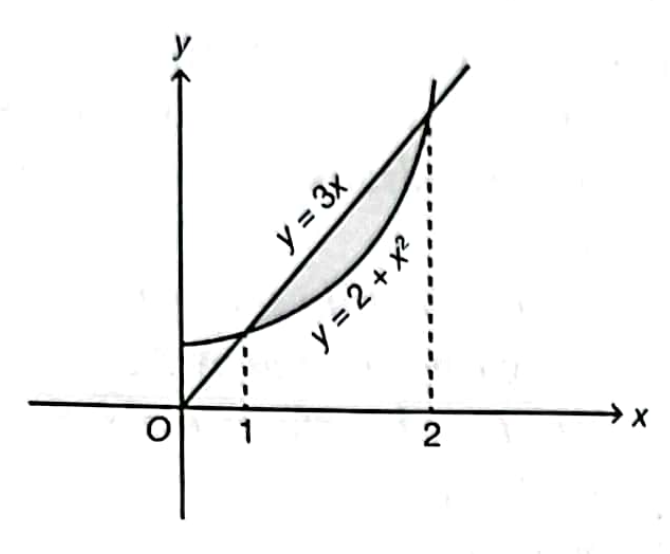
\includegraphics[width=0.3\textwidth,valign=t]{./images/21.png}
                  \end{enumerate}

            \item The region bounded by the curve $y = \dfrac{8}{x}$, the x-axis, and the
                  straight line $x = 2$ and $x = k$ is rotated through $360^\circ$ about the
                  x-axis as shown in the following diagram.
                  \begin{center}
                        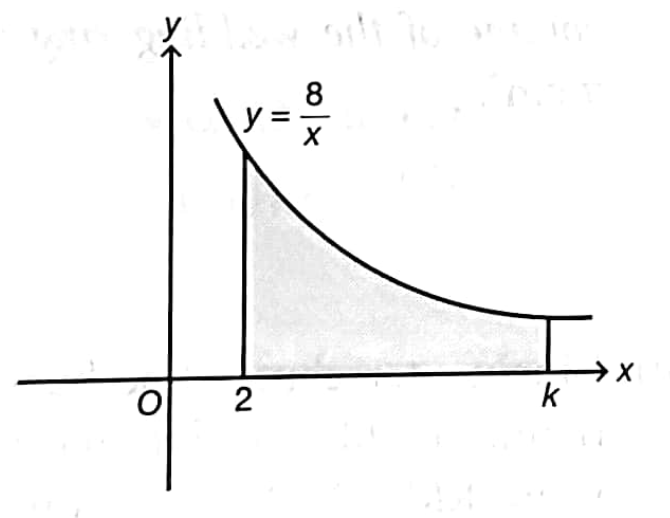
\includegraphics[width=0.3\textwidth,valign=t]{./images/22.png}
                  \end{center}
                  Express the volume generated by the region in terms of $k$. If the value of $k$ becomes extremely large, deduce the nearest value of volume.

            \item The following diagram shows a part of the curve $y =4 +3x - x^2$ and the
                  straight line $y = x+1$.
                  \begin{center}
                        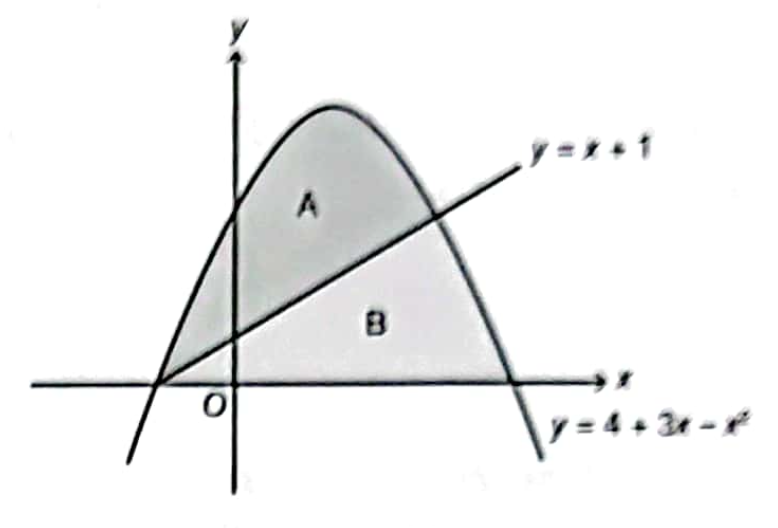
\includegraphics[width=0.3\textwidth,valign=t]{./images/23.png}
                  \end{center}
                  Find the ration of the area of the shaded region $A$ to the area of the shaded region $B$.

            \item The following diagram shows two curves $y = x^2 - 1$ and $y = 3+2x-x^2$.
                  \begin{center}
                        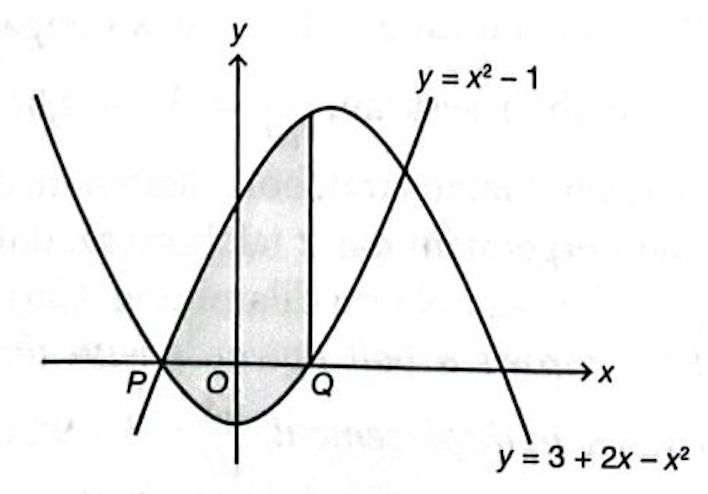
\includegraphics[width=0.3\textwidth,valign=t]{./images/24.png}
                  \end{center}
                  Find the coordinate of the points $P$ and $Q$. Hence, calculate the area of the shaded region.
      \end{enumerate}
\end{multicols*}

\end{document}